\def\year{2018}\relax
\documentclass[letterpaper]{article}
\usepackage{aaai18wip}
\usepackage{times}
\usepackage{helvet}
\usepackage{courier}
\usepackage{url}
\usepackage{graphicx}
\frenchspacing

%%%%% additional packages
\usepackage{mwe} %minipage
\usepackage{floatrow}
\frenchspacing  %Required
\usepackage[utf8]{inputenc} % allow utf-8 input
\usepackage[T1]{fontenc}    % use 8-bit T1 fonts
\usepackage{hyperref}       % hyperlinks
\usepackage{url}            % simple URL typesetting
\usepackage{booktabs}       % professional-quality tables
\usepackage{amsfonts}       % blackboard math symbols
\usepackage{nicefrac}       % compact symbols for 1/2, etc.
\usepackage{microtype}      % microtypography
\usepackage{balance}
\usepackage{amsmath}
\usepackage{subcaption}
\usepackage{mathrsfs} 
\usepackage{cancel}
\usepackage{amsfonts}
\usepackage[table]{xcolor}
\usepackage{titlesec}

\usepackage[]{algorithm2e}
\usepackage{framed}
\newcommand{\papertext}[1]{#1}
\newcommand{\techreport}[1]{}
\newcommand{\agp}[1]{\textcolor{magenta}{Aditya: #1}}
\newcommand{\dor}[1]{\textcolor{blue}{Doris: #1}}
\newcommand{\ads}[1]{\textcolor{green}{Akash: #1}}
\setcounter{secnumdepth}{2}

\usepackage{amsopn}
\DeclareMathOperator*{\argmax}{arg\,max}

\newcommand{\npar}{\par \noindent}
\newcommand{\stitle}[1]{\noindent \textbf{#1}}


\setlength{\pdfpagewidth}{8.5in}  %Required
\setlength{\pdfpageheight}{11in}  %Required
%PDF Info Is Required:
\pdfinfo{
/Title (Quality Evaluation Methods for Crowdsourced Image Segmentation)
/Author (Doris Jung-Lin Lee, Akash Das Sarma, Aditya Parameswaran)
/Keywords (Crowdsourcing, Human Computation, Image segmentation, Computer Vision)
}

\title{Quality Evaluation Methods for Crowdsourced Image Segmentation}
\setlength\titlebox{1.5in}   %squish author title height 
% The \author macro works with any number of authors. There are two
% commands used to separate the names and addresses of multiple
% authors: \And and \AND.
%
% Using \And between authors leaves it to LaTeX to determine where to
% break the lines. Using \AND forces a line break at that point. So,
% if LaTeX puts 3 of 4 authors names on the first line, and the last
% on the second line, try using \AND instead of \And before the third
% author name.
\begin{document}
           %\title{Quality Evaluation Methods for Crowdsourced Image Segmentation}
           \title{Aggregating Crowdsourced Image Segmentations}
           %\author{Doris Jung-Lin Lee, Akash Das Sarma, Aditya Parameswaran}
           % \numberofauthors{3}
            \author{%
              Doris Jung-Lin Lee\\
              University of Illinois, Urbana-Champaign\\
              jlee782@illinois.edu\\
            \And
              Akash Das Sarma\\
              Facebook, Inc.\\
              akashds@fb.com\\
            \And 
              Aditya Parameswaran\\
              University of Illinois, Urbana-Champaign\\
              adityagp@illinois.edu\\
            }
           \maketitle
           \begin{abstract}
           Instance-level image segmentation provides rich information crucial for scene understanding in a variety of real-world applications. In this paper, we evaluate multiple crowdsourced algorithms for the image segmentation problem, including novel worker-aggregation-based methods and retrieval-based methods from prior work. We characterize the different types of worker errors observed in crowdsourced segmentation, and present a clustering algorithm as a preprocessing step that is able to capture and eliminate errors arising due to workers having different semantic perspectives. We demonstrate that aggregation-based algorithms attain higher accuracies than existing retrieval-based approaches, while scaling better with increasing numbers of worker segmentations. 
           % Most large-scale image segmentation efforts such as MSCOCO have relied on computing a Jaccard metric against ground truth and retrieving the segmentation provided by the best worker. 
          \end{abstract}

%%%%%%%%%%%%%%%%%%%%%%%%% 01-Introduction %%%%%%%%%%%%%%%%%%%%%%%%%
%!TEX root = main.tex
\section{Introduction\label{sec:intro}}
Precise, instance-level object segmentation is crucial for identifying and tracking objects in a variety of real-world emergent applications of autonomy, including robotics~\cite{Natonek1998}, image organization and retrieval~\cite{Yamaguchi2012}, and medicine~\cite{Irshad2014}. To this end, there has been a lot of work on employing crowdsourcing to generate training data for segmentation, including Pascal-VOC~\cite{Everingham15}, LabelMe~\cite{Torralba2010}, OpenSurfaces~\cite{bell15minc}, and MS-COCO~\cite{Lin2012}. Unfortunately, raw data collected from the crowd is known to be noisy due to varying degrees of worker skills, attention, and motivation~\cite{bell14intrinsic,MDWWelinder2010}. 
\par To deal with these challenges, many have employed heuristics indicative of crowdsourced segmentation quality to pick the best worker-provided segmentation~\cite{Sorokin2008,Vittayakorn2011}. However, this approach ends up discarding the majority of the worker segmentations and is limited by what the best worker can do. In this paper, we make two contributions: First, we introduce a novel class of aggregation-based methods that incorporates portions of segmentations from multiple workers into a combined one described in Section~\ref{precision}. To our surprise, despite its intuitive simplicity, we have not seen this class of algorithms described or evaluated in prior work. We evaluate this class of algorithms against existing methods in Section~\ref{sec:experiment}. Second, our analysis of common worker errors in crowdsourced segmentation shows that workers often segment the wrong objects or erroneously include or exclude large semantically-ambiguous portions of an object in the resulting segmentation. We discuss such errors in Section~\ref{sec:error} and propose a clustering-based preprocessing technique that resolves them in Section~\ref{perspective}.%different worker perspectives in multiple segmentations.}
%To resolve semantic ambiguity and mistakes commonly observed in crowdsourced segmentation, we propose a clustering-based preprocessing technique that resolves different worker perspectives in multiple segmentations. 


%%%%%%%%%%%%%%%%%%%%%%%%%%%%%%%%%%%%%%%%%%%%%%%%%%%%%%%%%%%%%%%%%%%
%%%%%%%%%%%%%%%%%%%%%%%%% 02-RelatedWorks %%%%%%%%%%%%%%%%%%%%%%%%%

%!TEX root = main.tex
\begin{figure}
\centering
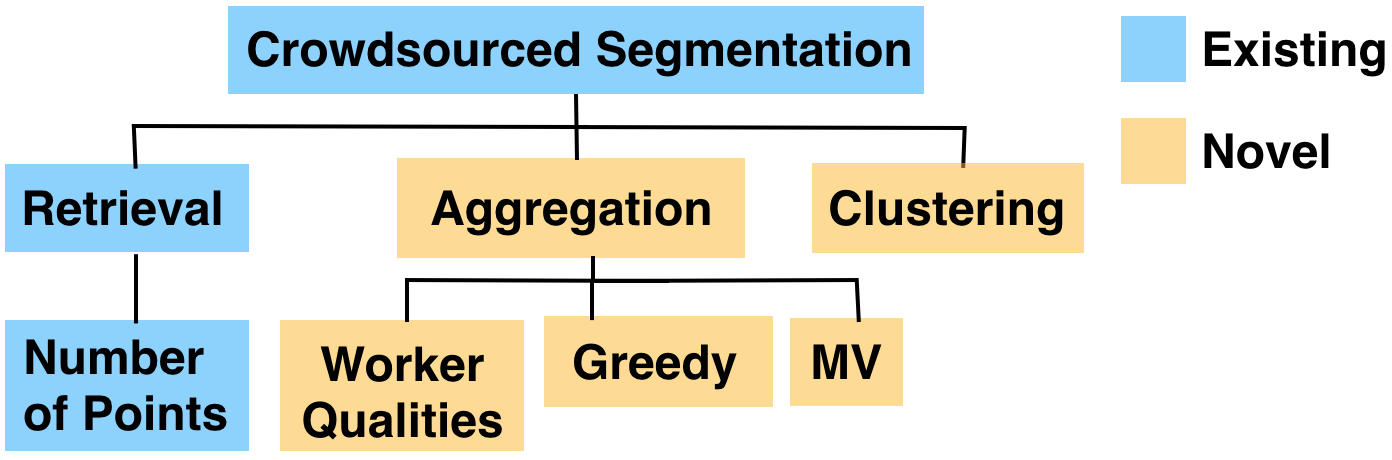
\includegraphics[width=0.7\linewidth]{plots/flowchart.png}
\caption{Taxonomy of quality evaluation algorithms for crowdsourced segmentation, including existing methods (blue) and our novel algorithms (yellow).
} %Majority-vote (MV) is colored both blue and yellow, since a common algorithm in crowdsourcing literature, but have not been extensively applied to crowdsourced image segmentation.}
%The crowdsourced approach can be largely classified as retrieval or aggregation-based methods. We further explore hybrid algorithms that makes use of signals that span over multiple categories, described in our technical report.
\label{flowchart}
\end{figure}
\section{Related Work\label{sec:related}}
%Many large-scale efforts in crowdsourced image segmentation contain little to no information on the quality characterization and evaluation of the collected dataset~\cite{Torralba2010,MartinFTM01,Li2009,Gurari2015}, which in dicate the lack of standardized approaches for quality evaluation. 
As shown in Figure \ref{flowchart}, quality evaluation methods for crowdsourced segmentation can be classified into two categories:

\stitle{Retrieval-based methods} pick the ``best'' worker segmentation based on some scoring criteria that evaluates the quality of each segmentation, including vision information~\cite{Vittayakorn2011,Russakovsky2015}, and click-stream behavior \cite{Cabezas2015,Sameki2015,Sorokin2008}.%expectation-maximization (EM) based approaches for bounding box quality estimation~\cite{OCWelinder2010}, 

\stitle{Aggregation-based methods} combine multiple worker segmentations to produce a final segmentation that is not restricted to any single worker segmentation. An aggregation-based majority vote approach was employed in Sameki et al. (\citeyear{Sameki2015}) to create an expert-established gold standard for characterizing their dataset and algorithmic accuracies, rather than for segmentation quality evaluation as described here.
%specialized segmentation interfaces or workflows that ensures that the annotations collected are of high quality, including 

% \par Orthogonal methods to improve segmentation quality include periodic verification~\cite{Lin2014,Everingham15}, specialized interfaces~\cite{Song2018}, and vision-based supervision~\cite{Russakovsky2015,Gurari2016}. These methods could be used for quality improvement on top of any of the algorithms in this paper.  %Since these policy-based methods are interface-dependent, require expensive expert-drawn ground-truth annotations or vision information, the results are not easily reproducible. In addition, the segmentations collected by the simple click-and-draw interface in many of the large scale segmentation efforts can not be improved with this technique as a post-processing method. Due to the lack of reproducibility, our paper do not compare against these policy-based methods in extensive details.



%%%%%%%%%%%%%%%%%%%%%%%%%%%%%%%%%%%%%%%%%%%%%%%%%%%%%%%%%%%%%%%%%%%
%%%%%%%%%%%%%%%%%%%%%%%%% 03-ErrorAnalysis %%%%%%%%%%%%%%%%%%%%%%%%%

%!TEX root = main.tex
\section{Error Analysis\label{sec:error}}
\par On collecting and analyzing a number of crowdsourced segmentations (described in Section~\ref{dataset}), we found that common worker segmentation errors can be classified into three types: (1) \textbf{Semantic Ambiguity:} workers have differing opinions on whether particular regions belong to an object (Figure~\ref{error_examples} left: annotations around `flower and vase' when `vase' is requested); (2) \textbf{Semantic Error:} workers annotate the wrong object entirely (Figure~\ref{error_examples} right: annotations around `turtle' and `monitor' when `computer' is requested.); and (3) \textbf{Boundary Imperfection:} workers make unintentional mistakes while drawing the boundaries, either due to low image resolution, small area of the object, or lack of drawing skills (Figure~\ref{tile_demo} left: imprecision around the `dog' object).
\par Quality evaluation methods in prior work have largely focused on minimizing boundary imperfection issues. So, we first describe our novel aggregation-based algorithms designed to reduce boundary imperfections in Section~\ref{precision}. Next, in Section~\ref{perspective}, we discuss a preprocessing method that eliminates semantic ambiguities and errors.
%, also observed in prior work~\cite{Sorokin2008,Lin2014,Gurari2018}.
We present our experimental evaluation in Section~\ref{sec:experiment}.
\begin{figure}[h!]
    \centering
    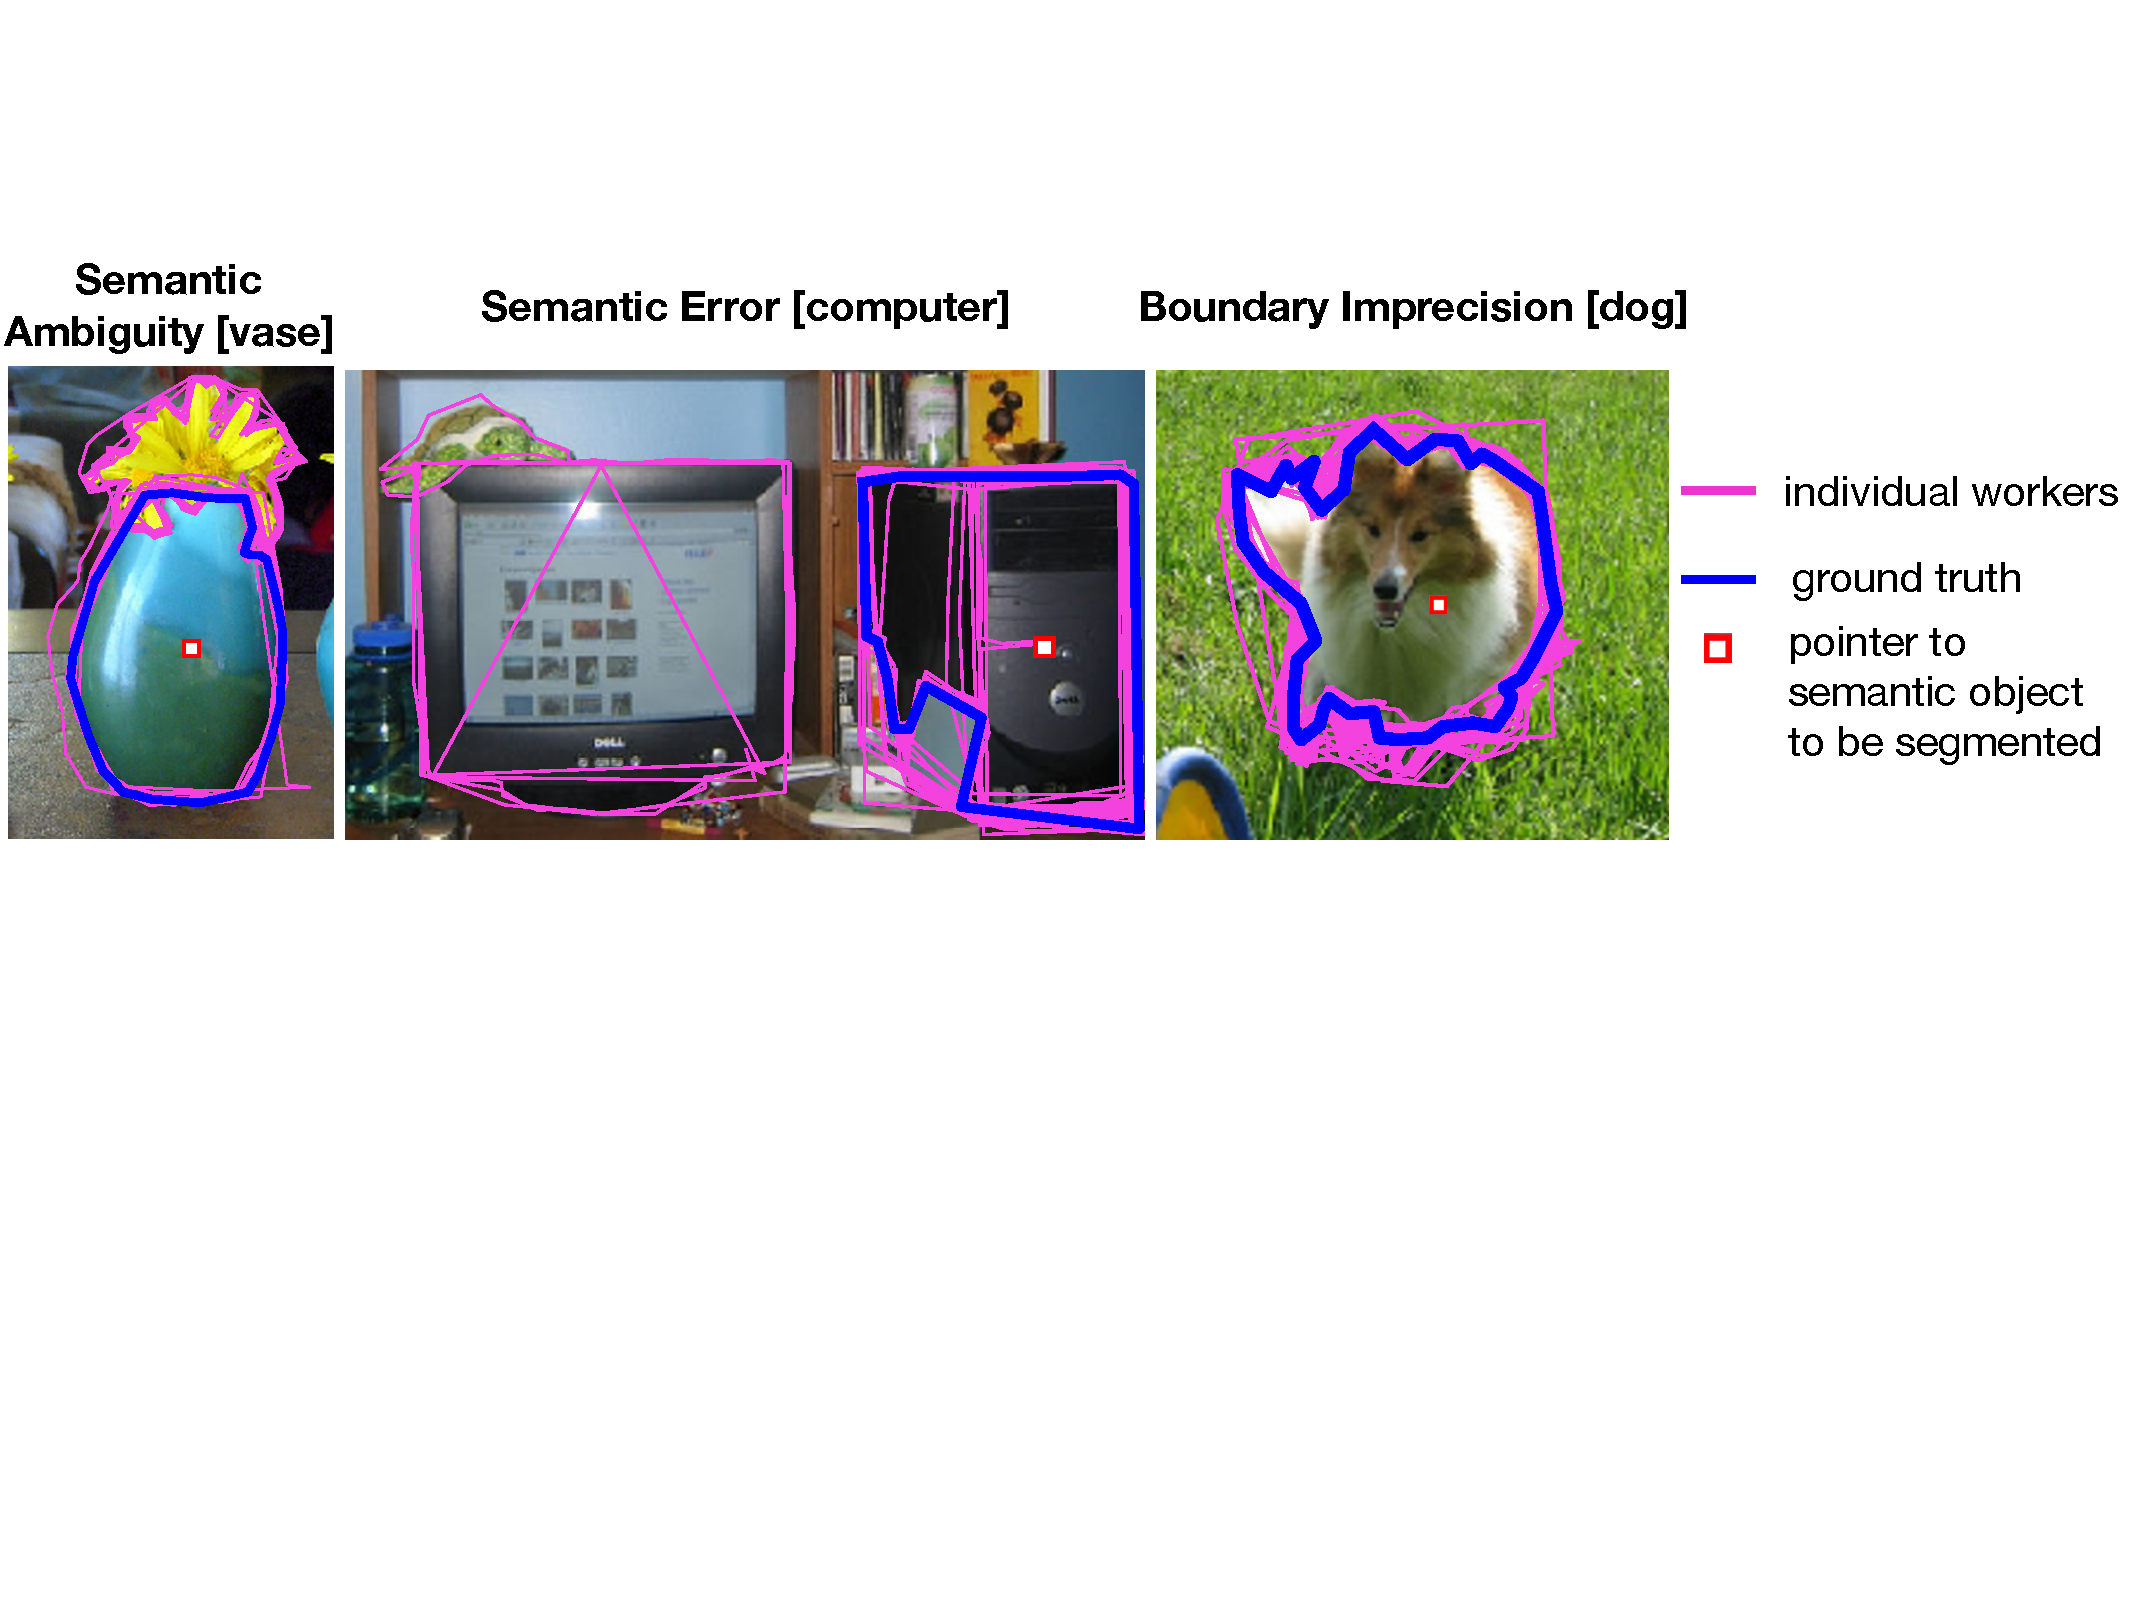
\includegraphics[width=\linewidth]{plots/errors.pdf}
    \caption{Examples of common worker errors.}
    \label{error_examples}
\end{figure}


%%%%%%%%%%%%%%%%%%%%%%%%%%%%%%%%%%%%%%%%%%%%%%%%%%%%%%%%%%%%%%%%%%%%%
%%%%%%%%%%%%%%%%%%%%%%%%% 04-PrecisionSavvy %%%%%%%%%%%%%%%%%%%%%%%%%

%!TEX root = main.tex
\section{Fixing Boundary Imperfections\label{precision}}
At the heart of our aggregation techniques is the \emph{tile data representation}. A tile is the smallest non-overlapping discrete unit created by overlaying all of the workers' segmentations on top of each other. 
The tile representation allows us to aggregate segmentations from multiple workers, rather than being restricted to a single worker's segmentation, allowing us to fix one worker's errors with help from another. In Figure \ref{tile_demo} (left), we display three worker segmentations for a toy example with 6 resulting tiles. Any subset of these tiles can contribute towards the final segmentation.
\par This simple but powerful idea of tiles also allows us to reformulate our problem from one of ``generating a segmentation'' to a setting that is much more familiar to crowdsourcing researchers. Since tiles are the lowest granularity units created by overlaying all workers' segmentations on top of each other, each tile is either completely contained within or outside a given worker segmentation. Specifically, we can regard a worker segmentation as multiple boolean responses where the worker has voted `yes' or `no' to every tile independently. Intuitively, a worker votes `yes' for every tile that is contained in their segmentation, and `no' for every tile that is not. As shown in Figure \ref{tile_demo} (right), tile $t_2$ is voted `yes' by worker 1, 2, and 3; tile $t_3$ is voted `yes' by worker 2 and 3. The goal of our aggregation algorithms is to pick an appropriate set of tiles that effectively trades off precision versus recall.
%\par Now, our problem of choosing a set of tiles to form a segmentation boils down to aggregating multiple boolean responses on every individual tile. Tiles with a final aggregated answer of ``yes'' are included in our output segmentation, while the remaining tiles are excluded. We should note that tiles need not necessarily be completely contained or completely outside the ground truth segmentation, therefore not every tile has a ground truth boolean answer. For tiles that are not completely contained or completely excluded in the ground truth, we gain recall but lose precision if we include them in our output segmentation, or lose recall and gain precision if we don't include them in our output segmentation. The goal of our aggregation algorithms, described below, is to pick a good set of tiles that effectively trade-off precision versus recall.
% The intuition here is that by splitting the image into tiles, we get finer granularity information than by looking at complete segmentations. This also allows us to aggregate data from multiple workers rather than having to choose a single worker bounding box---enabling the opportunity to choose partial segmentations by fixing one worker's errors via the help from another worker's segmentation.
% Now, we will describe several algorithms for picking a good set of tiles.
%The goal of our aggregation algorithms, described below, is to pick a good set of tiles that effectively trade-off precision versus recall.
\par Now that we have modeled segmentation as a collection of worker votes for tiles, we can now develop familiar variants of standard quality evaluation algorithms for this setting.

\stitle{Aggregation: Majority Vote Aggregation (MV)} 
\par \noindent This simple algorithm includes a tile in the output segmentation if and only if the tile has `yes' votes from at least 50\% of all workers. % segmentations.

\stitle{Aggregation: Expectation-Maximization (EM)}
\par \noindent Unlike MV, which assumes that all workers perform uniformly, EM approaches infer the likelihood that a tile is part of the ground truth segmentation, while simultaneously estimating hidden worker qualities.
In Section~\ref{sec:experiment} we evaluate an EM variant which assumes that each worker has a (different) fixed probability for a correct vote.
%is based on the probability that the worker will vote for a tile correctly. 
\techreport{Another model variant accounts for tile areas based on the intuition that workers should be penalized more if they make a mistake on a large tile (e.g. yellow tile in Figure \ref{tile_demo} middle) than on a small tile (e.g. orange tiles near the boundary in Figure \ref{tile_demo} middle). Our advanced %4-parameter Bernoulli 
worker quality model additionally accounts for true- and false-positive rates of the worker's tile votes.}
% Details of the formal derivation and other more fine-grained worker quality models can be found in our technical report.
Details of this, and more fine-grained variants can be found in our technical report.
%\agp{if we don't evaluate all of these we should drop these description. Also, cite the algo we are adopting in Sec 6.}

\stitle{Aggregation: Greedy Tile Picking (greedy)} 
%, and then picks tiles in that order, effectively picking tiles in order of their contribution to the Jaccard similarity against ground truth, 
\par \noindent The greedy algorithm picks tiles in descending order of the tiles' ratios of (estimated) overlap area with the ground truth to (estimated) non-overlap area with ground truth, for as long as the (estimated) Jaccard similarity of the resulting segmentation continues to increase. Intuitively, tiles that have a high overlap area and low non-overlap area contribute to high recall with limited loss of precision.
Since tile overlap and non-overlap areas, and Jaccard similarity of segmentations with ground truth are unknown, we use different heuristics to estimate these values. We discuss details of this algorithm and its theoretical guarantees in our technical report. 

\stitle{Retrieval: Number of Control Points (num pts)}
\par \noindent This algorithm picks the worker segmentation with the largest number of control points around the segmentation boundary (i.e., the most precise drawing) as the output segmentation \cite{Vittayakorn2011,Sorokin2008}.

\begin{figure}[h!]
\centering
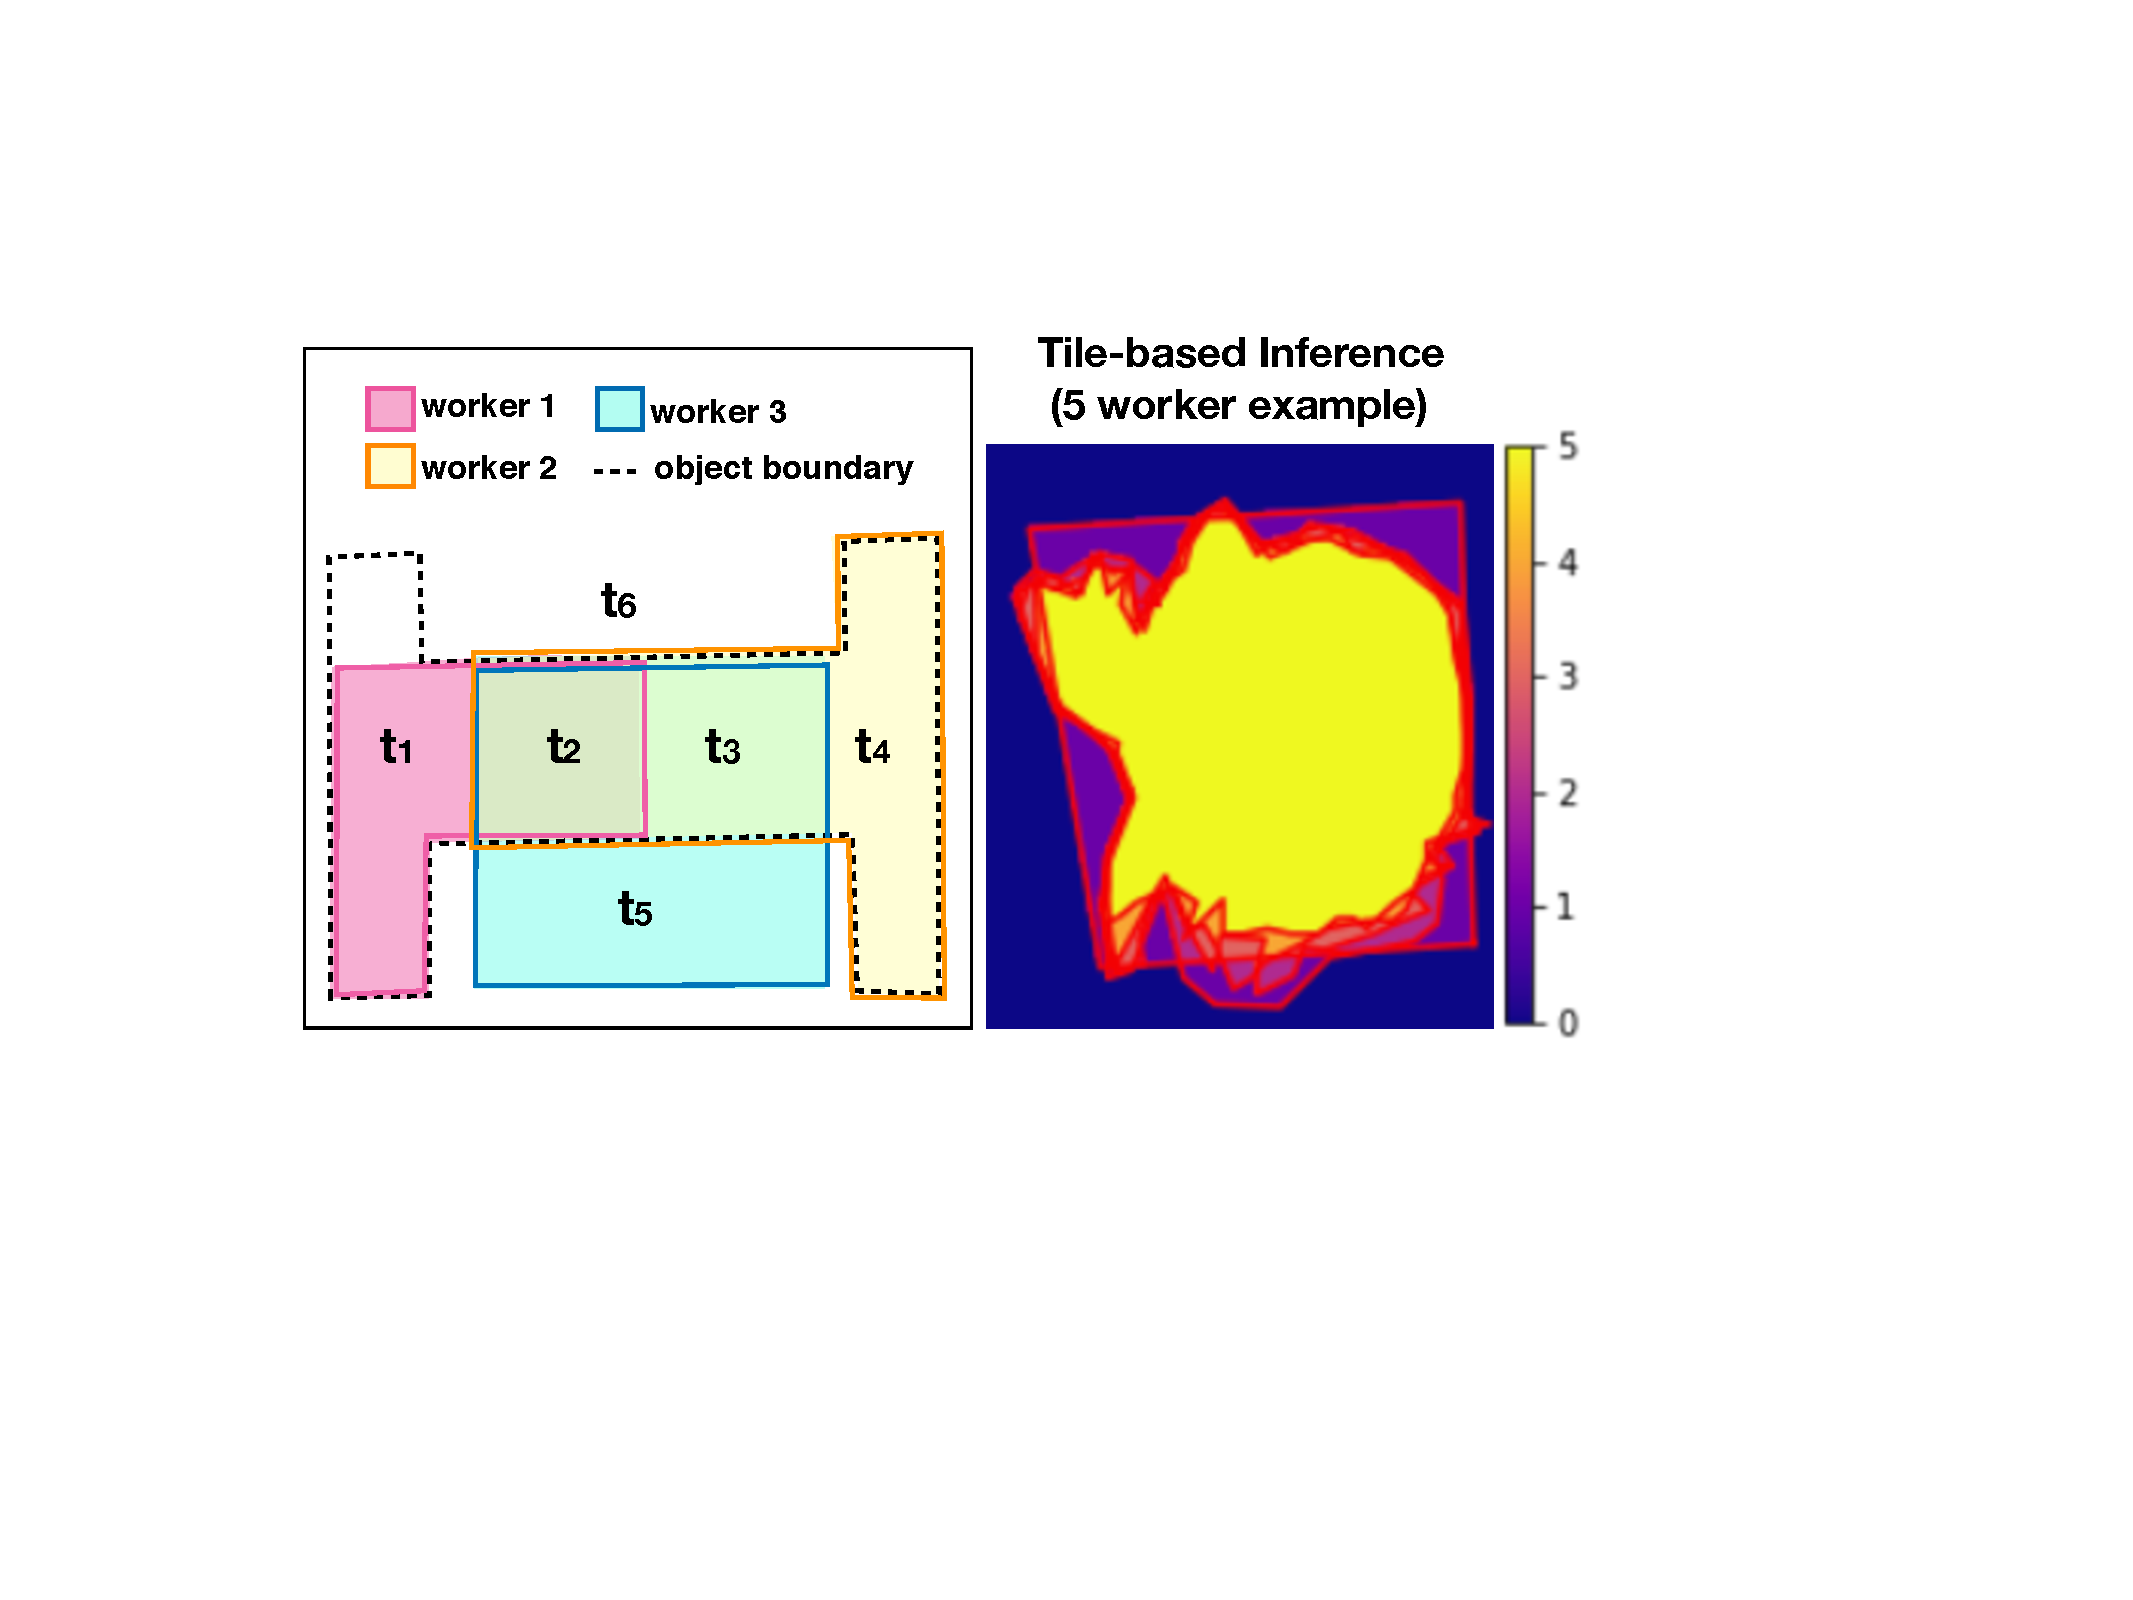
\includegraphics[width=0.8\linewidth]{plots/tile.pdf}
\caption{Left: Toy example demonstrating tiles created by three workers' segmentations around an object delineated by the black dotted line. Right: Segmentation boundaries drawn by five workers shown in red. Overlaid segmentation creates a mask where the color indicates the number of workers who voted for the tile region.}
\label{tile_demo}
\end{figure}  

%%%%%%%%%%%%%%%%%%%%%%%%%%%%%%%%%%%%%%%%%%%%%%%%%%%%%%%%%%%%%%%%%%%%%%%%%%%%%
%%%%%%%%%%%%%%%%%%%%%%%%% 05-Perspective_Clustering %%%%%%%%%%%%%%%%%%%%%%%%%
%!TEX root = main.tex
\section{Perspective Resolution\label{perspective}}
% \subsection{Worker Clustering}
As discussed in Section~\ref{sec:error}, disagreements often arise in segmentation due to differing worker perspectives on large tile regions. We developed a clustering-based preprocessing approach to resolve this issue.
% is based on the intuition that workers with similar perspectives  will have segmentations that are closer to each other. 
Based on the intuition that workers with similar perspectives will have segmentations that are close to each other, we compute the Jaccard similarity between each pair of segmentations and perform spectral clustering to separate the segmentations into clusters. Figure \ref{error_examples} (bottom) illustrates how spectral clustering divides the worker segmentations into clusters with meaningful semantic associations, reflecting the diversity of perspectives for the same task. Clustering results can be used as a preprocessing step for any quality evaluation algorithm by keeping only the segmentations that belong to the largest cluster, which is typically free of semantic errors.
\begin{figure}[h!]
  \centering
  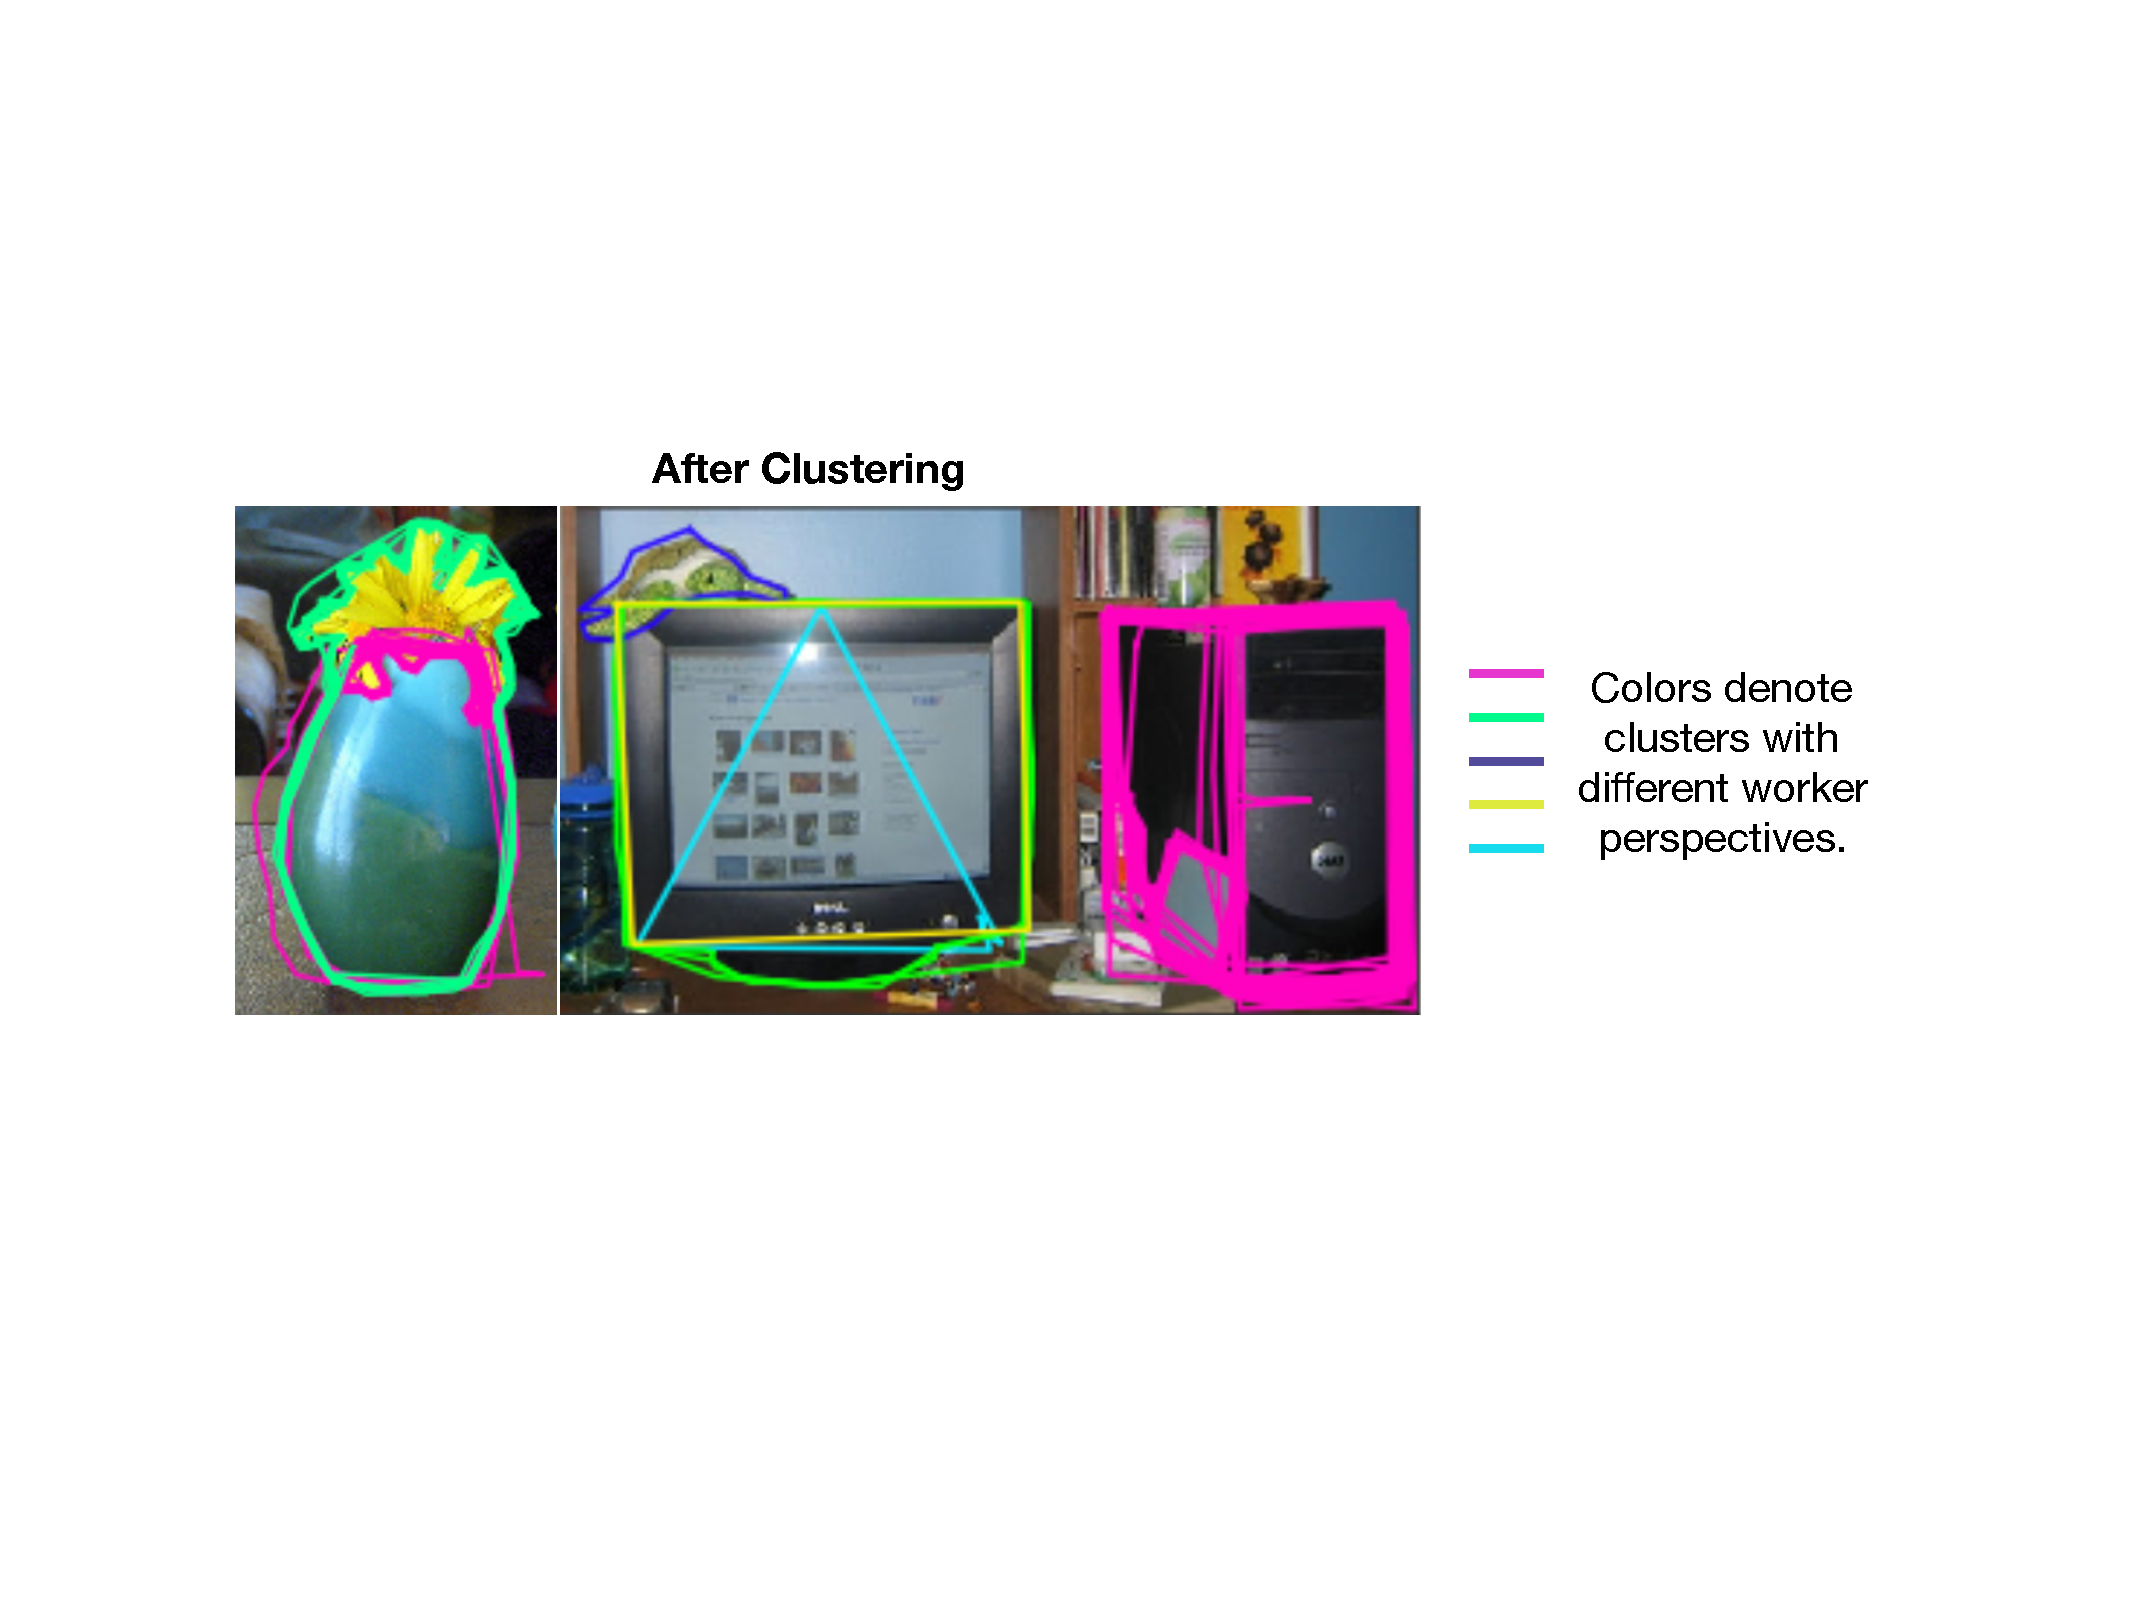
\includegraphics[width=0.9\linewidth]{plots/clustering.pdf}
  \caption{Example image showing clustering performed on the same object from Figure \ref{error_examples} left and middle.}
  \label{cluster_example}
\end{figure}
\par In addition, clustering offers the additional benefit of preserving a worker's semantic intentions. For example, while the green cluster in Figure~\ref{error_examples} (bottom right) would be considered \textit{bad} segmentations for the particular task (`computer'), this cluster can provide more data for another segmentation task corresponding to `monitor'. A potential future work direction would be to crowdsource the semantic labels for the computed clusters to enable the reuse of segmentations across multiple objects to lower costs.%the cost of data collection. %(which is cheaper and more accurate than segmentation)
%A potential future work includes adding additional crowdsourcing tasks for semantic labeling of clusters (which is cheaper and more accurate than segmentation) to enable reuse of annotations across multiple objects and lower the cost of data collection. 

%%%%%%%%%%%%%%%%%%%%%%%%%%%%%%%%%%%%%%%%%%%%%%%%%%%%%%%%%%%%%%%%%%%%%%%%%%%%%%
%%%%%%%%%%%%%%%%%%%%%%%%% 06-DatasetMetricEvaluation %%%%%%%%%%%%%%%%%%%%%%%%%
%!TEX root = main.tex
\section{Experimental Evaluation\label{sec:experiment}}

\stitle{Dataset Description\label{dataset}}
\par \noindent We collected crowdsourced segmentations from Amazon Mechanical Turk; each HIT consisted of one segmentation task for a specific pre-labeled object in an image. Workers were compensated \$0.05 per task. There were a total of 46 objects in 9 images from the MSCOCO dataset~\cite{Lin2014} segmented by 40 different workers each, resulting in a total of 1840 segmentations. Each task contained a keyword for the object and a pointer indicating the object to be segmented. Two of the authors generated the ground truth segmentations by carefully segmenting the objects using the same interface. %segmented the objects using our own segmentation interface and use the generated segmentations as ground truth data.%\agp{How did you get GT?} \dor{I just annotated very carefully to draw around the object as the GT, could not use the COCO annotations because of the semantic segmentation they used were different, so there ends up being a lot of semantic ambiguity. We should probably not get into the details here.}%These tasks represent a diverse set of task difficulty (different levels of clutteredness, occlusion, lighting) and levels of task ambiguity. 
\techreport{\par A sub-sampled dataset was created from the full dataset to determine the efficacy of these algorithms on varying number of worker responses. Every object was randomly sampled worker with replacement. For small worker samples, we average our results over larger number of batches than for large worker samples (which have lower variance, since the sample size is close to the original data size).}

\stitle{Evaluation Metrics}
\par \noindent Evaluation metrics used in our experiments measure how well the final segmentation (S) produced by these algorithms compare against ground truth (GT). We use the Jaccard score $\text{Jaccard (J)} = \frac{UA(S)}{IA(S)}$, which accounts for the intersection area, $IA=area(S\cap GT)$ and union area, $UA=area(S\cup GT)$ between the worker and ground truth segmentations.

\stitle{Experiment 1: Aggregation-based methods perform significantly better than retrieval-based methods}
\begin{figure}[h!]
   \centering
   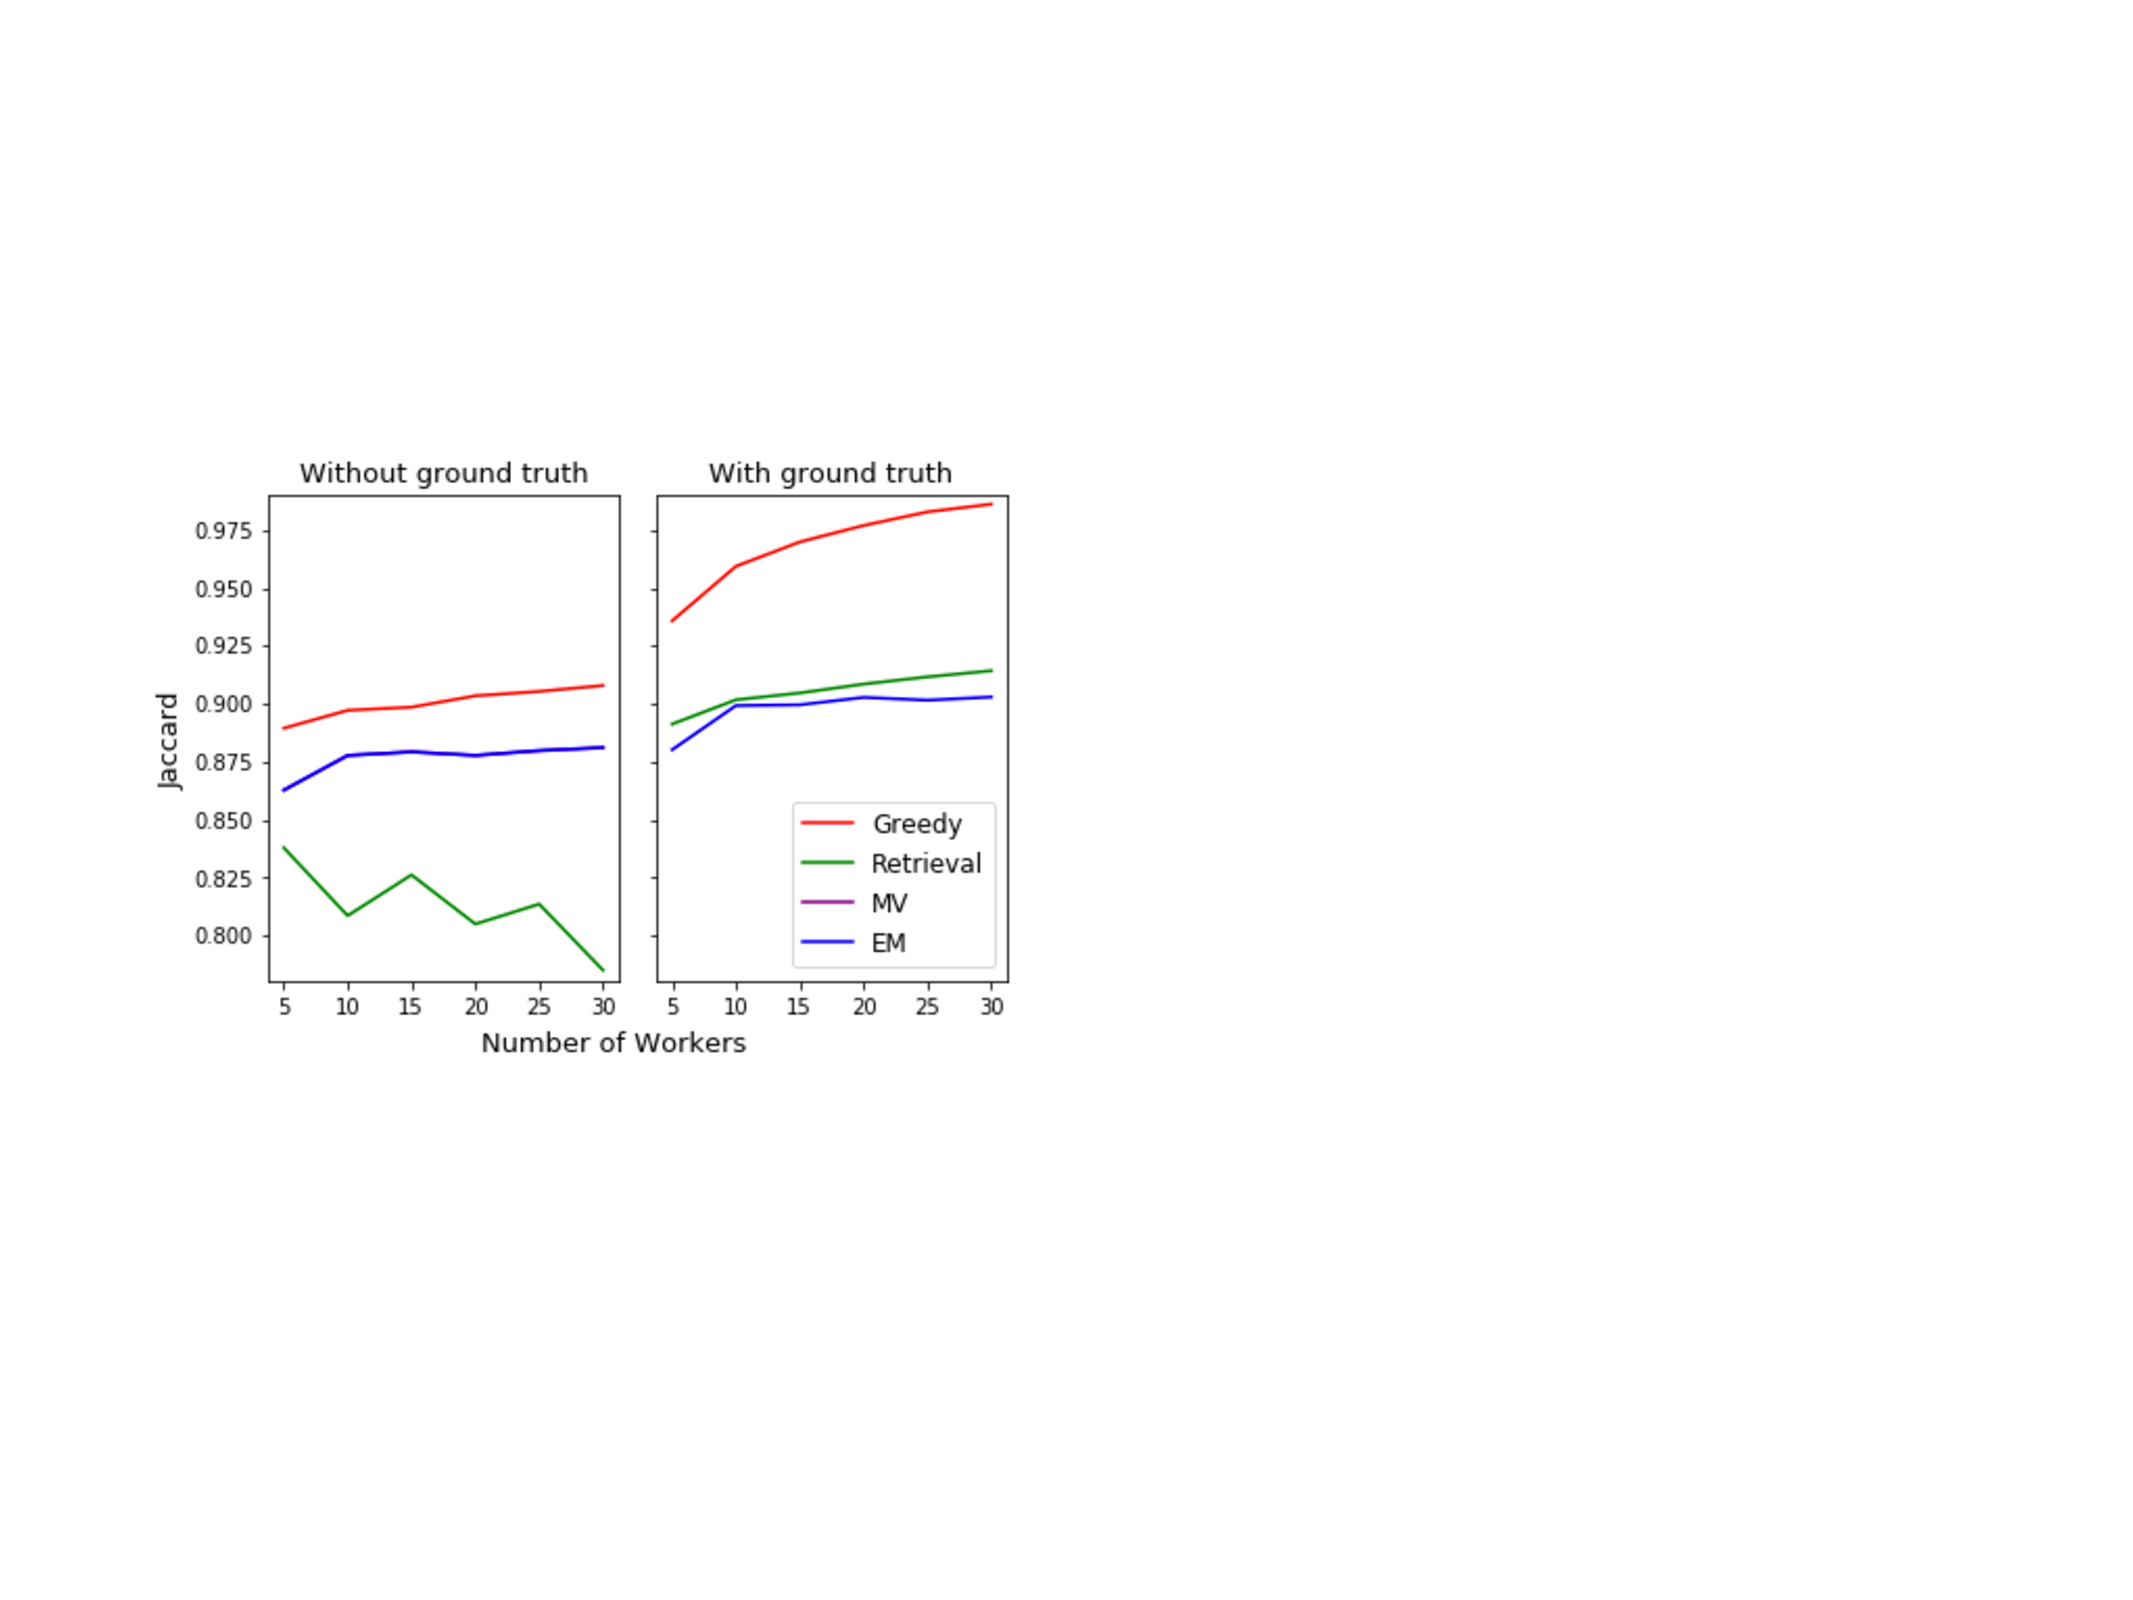
\includegraphics[width=0.75\textwidth]{plots/Retrieval_vs_Aggregation.pdf}
   \caption{Performance of the original algorithms that do not make use of ground truth information (Left) and ones that do (Right). Here, the EM result overlaps with MV as they exhibit similar performance. Other diverging variants of EM is described in our technical report.} %\agp{Explain setup for this. How did you generate this?} \dor{not sure what aditya means?}}%Performance comparison between best-performing retrieval and aggregation-based methods. 
   \label{retrieval_vs_aggregation}   
\end{figure} 
\npar In Figure~\ref{retrieval_vs_aggregation}, we vary the number of worker segmentations along the x-axis and plot the average Jaccard score on the y-axis across different worker samples of a given size across different algorithms. Figure~\ref{retrieval_vs_aggregation} (left) shows that the performance of aggregation-based algorithms (greedy, EM) exceeds the best achievable through existing retrieval-based methods (Retrieval). Then, in Figure \ref{retrieval_vs_aggregation} (right), we estimate the upper-bound performance of each algorithm by assuming that `full information' based on ground truth is given to the algorithm. For greedy, the algorithm is aware of all the actual tile overlap and non-overlap areas against ground truth. %, and does not need to approximate these values.
For EM, %we consider the performance of the algorithm if 
the true worker quality parameter values (under our worker quality model) are known. For retrieval, the full information version directly picks the worker with the highest Jaccard similarity with respect to the ground truth. By making use of ground truth information (Figure~\ref{retrieval_vs_aggregation} right), the best aggregation-based algorithm can achieve a close-to-perfect average Jaccard score of 0.98 as an upper bound, far exceeding the results achievable by any single `best' worker (J=0.91). This result demonstrates that aggregation-based methods are able to achieve better performance by performing inference at the tile granularity, which is guaranteed to be finer grained than any individual worker segmentation. 

\stitle{The performance of aggregation-based methods scale well as more worker segmentations are added.}
\par \noindent Intuitively, larger numbers of worker segmentations result in finer granularity tiles for the aggregation-based methods. The first row in Table~\ref{statsTable} shows the average percentage change in performance between 5-workers and 30-workers samples. We observe that aggregation based methods typically improve in performance with an increase in number of workers, while this is not generally true for retrieval-based methods.

\stitle{Experiment 2: Clustering as preprocessing improves algorithmic performance.}
\par \noindent The second row in Table~\ref{statsTable} shows the average percentage Jaccard change when clustering preprocessing is used. While clustering generally results in an accuracy increase, since the `full information' variants are already free of semantic errors, we do not see further improvement for these variants. %In particular, we see a greater improvement with clustering preprocessing for algorithms that are not very robust in resolving semantic errors or ambiguity, such as for the \texttt{num pts} retrieval algorithm, than compared to the aggregation-based methods. 
%\agp{Weird, this is experiment 2. Divide this up into two parts. (Right now it seems as if all findings are from Fig 4, so this comes as a surprise.)}\dor{should we divide table~\ref{statsTable} into two separate tables?}
\begin{table}[h!]
   \small
     \setlength\tabcolsep{1.5pt}
      \begin{tabular}{l|l|l|l|l|l|l}
         & \multicolumn{2}{c|}{Retrieval-based} & \multicolumn{4}{l}{Aggregation-based} \\ \hline
      Algorithm         & num pts         & worker*        & MV    & EM    & greedy  & greedy*  \\ \hline
      Worker Scaling    & -6.30           & 2.58               & 2.12  & 1.78  & 2.07   & 5.38        \\ \hline
      Clustering Effect & 5.92            & -0.02              & 2.05  & 0.03  & 5.73    & 0.283       
      \end{tabular}
      \caption{Jaccard percentage change due to worker scaling and clustering. Algorithms with * use ground truth information.}
      \label{statsTable}
\end{table}


%%%%%%%%%%%%%%%%%%%%%%%%%%%%%%%%%%%%%%%%%%%%%%%%%%%%%%%%%%%%%%%%%%%
%%%%%%%%%%%%%%%%%%%%%%%%% 07-FutureWork %%%%%%%%%%%%%%%%%%%%%%%%%%%
%!TEX root = main.tex 
\section{Conclusion and Future Work}
We identified three different types of errors for crowdsourced image segmentation, developed a clustering-based method to capture the semantic diversity caused by differing worker perspectives, and introduced novel aggregation-based methods that produce more accurate segmentations than existing retrieval-based methods.
\par Our preliminary studies show that our worker quality models are good indicators of the actual accuracy of worker segmentations. We also observe that the greedy algorithm is capable of achieving close-to-perfect segmentation accuracy with ground truth information. Given the success of aggregation-based methods, including the simple majority vote algorithm, we plan to use our worker quality insights to improve our EM and greedy algorithms. 
We are also working on using computer vision signals to further improve our algorithms.
% Bridging the gap between our current approach to the maximum potential of aggregation-based methods can result in more accurate and perspective-aware crowdsourced segmentation outputs in the future.


%%%%%%%%%%%%%%%%%%%%%%%%%%%%%%%%%%%%%%%%%%%%%%%%%%%%%%%%%%%%%%%%%%%
\balance  
\bibliographystyle{named}
\bibliography{reference}
\end{document}
